\documentclass[aspectratio=169,10pt]{beamer}

\usepackage[default]{sourcesanspro}
\usepackage{fontawesome5}
\usepackage{booktabs}
\usepackage{tabularx}
\usepackage{array}
\usepackage{tikz}
\usetikzlibrary{arrows.meta,positioning}
\usepackage{graphicx}

\definecolor{Navy}{HTML}{17324D}
\definecolor{Blue}{HTML}{247BA0}
\definecolor{Teal}{HTML}{20A39E}
\definecolor{Amber}{HTML}{E09F3E}
\definecolor{Red}{HTML}{C94C4C}
\definecolor{Ink}{HTML}{243447}
\definecolor{Muted}{HTML}{64748B}
\definecolor{Mist}{HTML}{E8EEF2}
\definecolor{Wash}{HTML}{F5F8FA}
\definecolor{PaleTeal}{HTML}{E7F7F5}
\definecolor{PaleAmber}{HTML}{FFF4E3}
\definecolor{PaleRed}{HTML}{FCECEC}

\setbeamercolor{normal text}{fg=Ink,bg=white}
\setbeamercolor{frametitle}{fg=Navy,bg=white}
\setbeamercolor{structure}{fg=Teal}
\setbeamerfont{frametitle}{size=\Large,series=\bfseries}
\setbeamertemplate{navigation symbols}{}
\setbeamersize{text margin left=0.60cm,text margin right=0.60cm}
\setbeamertemplate{frametitle}{%
  \vspace{0.20cm}\insertframetitle\par
  \vspace{-0.12cm}\color{Teal}\rule{1.05cm}{1.5pt}\color{Mist}\rule{\dimexpr\textwidth-1.05cm\relax}{1.5pt}}
\setbeamertemplate{footline}{%
  \leavevmode\hbox{%
    \begin{beamercolorbox}[wd=.78\paperwidth,ht=2.7ex,dp=1.1ex,leftskip=.60cm]{normal text}%
      \color{Muted}\scriptsize FOR2107 × Tozzi · preliminary · 23 July 2026
    \end{beamercolorbox}%
    \begin{beamercolorbox}[wd=.22\paperwidth,ht=2.7ex,dp=1.1ex,rightskip=.60cm plus1fil]{normal text}%
      \color{Muted}\scriptsize\insertframenumber/6
    \end{beamercolorbox}}}

\newcommand{\kpi}[2]{%
  \begin{minipage}[c][0.82cm][c]{0.22\textwidth}\centering
    {\color{Navy}\fontsize{22}{22}\selectfont\bfseries #1}\\[1pt]
    {\color{Muted}\scriptsize\MakeUppercase{#2}}
  \end{minipage}}
\newcommand{\matchmark}{\color{Teal}\faCheckCircle}
\newcommand{\partialmark}{\color{Amber}\faExclamationCircle}
\newcommand{\missingmark}{\color{Red}\faTimesCircle}
\newcommand{\pendingmark}{\color{Muted}\faMinusCircle}

\begin{document}

% ---------------------------------------------------------------------------
\setbeamertemplate{background}{\includegraphics[width=\paperwidth,height=\paperheight]{figures/title_background.png}}
\setbeamertemplate{footline}{}
\begin{frame}[plain]
  \begin{tikzpicture}[remember picture,overlay]
    \fill[Navy,opacity=.18] (current page.south west) rectangle (current page.north east);
    \node[anchor=west,text width=8.05cm] at ([xshift=.78cm,yshift=.42cm]current page.west) {%
      {\color{Teal}\small\bfseries PRELIMINARY RESULTS \;·\; SCIENTIFIC ADVISORY UPDATE}\par
      \vspace{0.24cm}
      {\color{white}\fontsize{31}{33}\selectfont\bfseries FOR2107\\First results}\par
      \vspace{0.20cm}
      {\color{white!76}\large Progress toward reproducing the Tozzi framework}\par
      \vspace{0.54cm}
      {\color{white!70}\small 75 scans \;·\; 67 selected participants \;·\; first circuit profiles}\par
      \vspace{0.66cm}
      {\color{white!62}\scriptsize 23 July 2026 \hspace{0.35cm} | \hspace{0.35cm} What the first evidence shows}
    };
  \end{tikzpicture}
\end{frame}
\setbeamertemplate{background}{}
\setbeamertemplate{footline}{%
  \leavevmode\hbox{%
    \begin{beamercolorbox}[wd=.78\paperwidth,ht=2.7ex,dp=1.1ex,leftskip=.60cm]{normal text}\color{Muted}\scriptsize FOR2107 × Tozzi · preliminary · 23 July 2026\end{beamercolorbox}%
    \begin{beamercolorbox}[wd=.22\paperwidth,ht=2.7ex,dp=1.1ex,rightskip=.60cm plus1fil]{normal text}\color{Muted}\scriptsize\insertframenumber/6\end{beamercolorbox}%
  }}

% ---------------------------------------------------------------------------
\begin{frame}{The scientific idea}
\centering
\begin{tikzpicture}[
  node distance=.48cm,
  box/.style={rounded corners=4pt,minimum height=1.55cm,text width=2.75cm,align=center,fill=Wash,draw=Mist,line width=.7pt,font=\small},
  arrow/.style={-{Stealth[length=2.5mm]},line width=1.1pt,color=Teal}
]
  \node[box] (scan) {\color{Blue}\faBrain\\[2pt]\textbf{Measure the brain}\\{\scriptsize task-free scan\\emotion tasks\\Go/NoGo task\\}};
  \node[box,right=of scan] (profile) {\color{Teal}\faProjectDiagram\\[2pt]\textbf{Build one profile}\\{\scriptsize compare with healthy controls\\}};
  \node[box,right=of profile] (groups) {\color{Blue}\faUsers\\[2pt]\textbf{Find shared patterns}\\{\scriptsize people with similar profiles\\}};
  \node[box,right=of groups] (meaning) {\color{Teal}\faHeartbeat\\[2pt]\textbf{Test clinical value}\\{\scriptsize symptoms · behavior · treatment\\}};
  \draw[arrow] (scan)--(profile); \draw[arrow] (profile)--(groups); \draw[arrow] (groups)--(meaning);
\end{tikzpicture}

\vspace{.62cm}
\begin{beamercolorbox}{block body}
  \centering
  {\color{Navy}\large\bfseries Can brain-circuit patterns reveal clinically meaningful subgroups?}\par
  \vspace{.14cm}
  {\small Tozzi et al. answered this using a large sample and several scan conditions. Our current analysis tests the same idea using resting-state scans first.\par}
\end{beamercolorbox}
\end{frame}

% ---------------------------------------------------------------------------
\begin{frame}{Where the project stands today}
\centering
\begin{beamercolorbox}[rounded=true,sep=.12cm,wd=.96\textwidth]{block body}
  \kpi{75}{resting-state scans}\kpi{67}{selected participants}\kpi{17}{clinical}\kpi{50}{healthy controls}
\end{beamercolorbox}

\vspace{.48cm}
\begin{columns}[T,onlytextwidth]
  \begin{column}{.31\textwidth}
    \begin{beamercolorbox}[rounded=true,sep=.30cm]{block body}
      {\color{Teal}\large\faCheckCircle}\hspace{.12cm}{\color{Navy}\bfseries Achieved}\par\vspace{.18cm}
      \small Resting-state circuit profiles can now be produced for every available participant.
    \end{beamercolorbox}
  \end{column}
  \begin{column}{.31\textwidth}
    \begin{beamercolorbox}[rounded=true,sep=.30cm]{block body}
      {\color{Amber}\large\faEye}\hspace{.12cm}{\color{Navy}\bfseries First evidence}\par\vspace{.18cm}
      \small Different average circuit patterns appear when groups are formed.
    \end{beamercolorbox}
  \end{column}
  \begin{column}{.31\textwidth}
    \begin{beamercolorbox}[rounded=true,sep=.30cm]{block body}
      {\color{Red}\large\faHourglassHalf}\hspace{.12cm}{\color{Navy}\bfseries Still needed}\par\vspace{.18cm}
      \small Task scans, motion assessment, and a larger clinical sample.
    \end{beamercolorbox}
  \end{column}
\end{columns}

\vspace{.48cm}

\begin{tikzpicture}
  \fill[PaleAmber,rounded corners=4pt] (0,0) rectangle (14.7,.78);
  \node[anchor=west,text width=14cm] at (.30,.39) {\color{Navy}\small\textbf{Bottom line:} the measurement workflow is ready; the evidence for reproducible patient subgroups is not.};
\end{tikzpicture}
\end{frame}

% ---------------------------------------------------------------------------
\begin{frame}{What the first results show}
\centering
\includegraphics[width=.85\textwidth]{figures/preliminary_results_v3.pdf}

\vspace{.08cm}
\begin{columns}[T,onlytextwidth]
  \begin{column}{.47\textwidth}
    \begin{beamercolorbox}[rounded=true,sep=.25cm]{block body}
      {\color{Teal}\faCheckCircle}\hspace{.12cm}{\color{Navy}\bfseries Observable}\par\vspace{.10cm}
      \small The available data produce distinct average circuit patterns.
    \end{beamercolorbox}
  \end{column}
  \begin{column}{.47\textwidth}
    \begin{beamercolorbox}[rounded=true,sep=.25cm]{block body}
      {\color{Red}\faTimesCircle}\hspace{.12cm}{\color{Navy}\bfseries Not established}\par\vspace{.10cm}
      \small Separation is not stronger than chance, groups are small, and symptoms do not differ reliably.
    \end{beamercolorbox}
  \end{column}
\end{columns}

\end{frame}

% ---------------------------------------------------------------------------
\begin{frame}{How far are we from the published result?}
\small
\renewcommand{\arraystretch}{1.30}
\setlength{\tabcolsep}{3pt}
\centering
\begin{tabular}{>{\raggedright\arraybackslash\bfseries\color{Navy}}m{2.55cm} >{\raggedright\arraybackslash}m{5.10cm} >{\raggedright\arraybackslash}m{5.25cm} >{\centering\arraybackslash}m{.55cm}}
  \toprule
  & \multicolumn{1}{c}{\textbf{Tozzi et al.}} & \multicolumn{1}{c}{\textbf{Current evidence}} & \\
  \midrule
  Evidence base & 801 clinical participants; several studies & 17 clinical participants; one current sample & \partialmark \\
  Brain information & Rest, emotion, and cognitive control & Resting-state information only & \partialmark \\
  Shared principle & Each person summarized by a circuit profile & Same person-level profile concept & \matchmark \\
  Confidence & Repeated and independent confirmation & No independent confirmation yet & \partialmark \\
  Conclusion & Six clinically distinct subgroups & \textbf{No replicated subgroup yet} & \pendingmark \\
  \bottomrule
\end{tabular}

\vspace{.34cm}
{\large\color{Navy}\textbf{The framework matches; the finding is not yet replicated.}}

\end{frame}

% ---------------------------------------------------------------------------
\begin{frame}{What would change the conclusion?}
\begin{columns}[T,onlytextwidth]
  \begin{column}{.31\textwidth}
    \begin{beamercolorbox}[rounded=true,sep=.32cm]{block body}
      \centering{\color{Blue}\Large\faDatabase}\par\vspace{.14cm}
      {\color{Navy}\large\bfseries Complete the evidence}\par\vspace{.14cm}
      \small Full participant set, task-based measures, and motion assessment.
    \end{beamercolorbox}
  \end{column}
  \begin{column}{.31\textwidth}
    \begin{beamercolorbox}[rounded=true,sep=.32cm]{block body}
      \centering{\color{Amber}\Large\faVials}\par\vspace{.14cm}
      {\color{Navy}\large\bfseries Challenge the result}\par\vspace{.14cm}
      \small Show that the same patterns persist across samples and analysis choices.
    \end{beamercolorbox}
  \end{column}
  \begin{column}{.31\textwidth}
    \begin{beamercolorbox}[rounded=true,sep=.32cm]{block body}
      \centering{\color{Teal}\Large\faHeartbeat}\par\vspace{.14cm}
      {\color{Navy}\large\bfseries Show clinical value}\par\vspace{.14cm}
      \small Demonstrate reliable differences in symptoms, behavior, or treatment response.
    \end{beamercolorbox}
  \end{column}
\end{columns}

\vspace{.48cm}
\begin{beamercolorbox}[rounded=true,sep=.30cm]{block body}
  {\color{Amber}\bfseries One design decision remains:}\quad
  \small without a direct Go/NoGo equivalent, define the goal as either a \textbf{partial replication} or a \textbf{scientific extension using the closest available task} before analyzing task data.
\end{beamercolorbox}

\vspace{.45cm}

\begin{tikzpicture}
  \fill[Navy,rounded corners=4pt] (0,0) rectangle (14.7,1.02);
  \node[anchor=west,text width=14cm] at (.30,.51) {\color{white}\large\textbf{Current assessment:} feasibility demonstrated; replication evidence pending.};
\end{tikzpicture}
\end{frame}

\end{document}
